% !TEX root = ../distCjHMSC.tex
%================================
The results of this section report the estimation for the eight locations given in the table \ref{tab:sensor-specifications}.


%================================
\section{Results of IS26}
%================================
In this section we report analysis of the data from IS2. The numerical values are reported in figures from \ref{fig:C2} to \ref{fig:C8} associated with the sensors 1 to 8.

 \figscale{3monthsonIS26SUT1.png}{Couple H1C1}{fig:C1}{1}
 
 \figscale{3monthsonIS26SUT2.png}{Couple H2C2}{fig:C2}{1}
  \figscale{3monthsonIS26SUT3.png}{Couple H3C3}{fig:C3}{1}

 \newpage
 \figscale{3monthsonIS26SUT4.png}{Couple H4C4}{fig:C4}{1}
 \figscale{3monthsonIS26SUT5.png}{Couple H5C5}{fig:C5}{1}

 \newpage
 \figscale{3monthsonIS26SUT6.png}{Couple H6C6}{fig:C6}{1}
 \figscale{3monthsonIS26SUT7.png}{Couple H7C7}{fig:C7}{1}

 \newpage
  \figscale{3monthsonIS26SUT8.png}{Couple H8C8}{fig:C8}{1}



%================================
\newpage\clearpage
%================================
%================================
\section{Comments}
%================================
\subsection{About the selected MSC threshold}
%================================
We said that we can not choose a too low value for the MSC threshold because the underdetermination. That appears clearly on figure \ref{fig:afewdaysonI26C6H6twoMSC}.
When the  MSC threshold is $0.7$, there is a large discrepancy between the estimated ratios, see \eqref{eq:estimated-Ratio} and we outline that there is no way to solve the underdetermination. But for an MSC threshold of $0.95$, the two curves are very close.

\figscale{afewdaysonI26C6H6twoMSC.pdf}{Couple H6C6, for two MSC thresholds.}{fig:afewdaysonI26C6H6twoMSC}{0.7}

On the other hand if the ratio between the two noise levels are perfectly known the indetermination is removed and we can use formula \eqref{eq:known-noise-ratio}. You might be tempted to say that the two noises on the two sensors are identical except theirs levels and consider that the ratio is given by the number of inlets in the noise reduction system. However the figure \ref{fig:afewdaysonI26C4H4knownnoiseratio} shows that the curve with a MSC threshold of $0.5$ and the formula \eqref{eq:known-noise-ratio} lead to values different from the curves obtained with a a MSC threshold of $0.95$.

\figscale{afewdaysonI26C4H4knownnoiseratio.pdf}{Couple H4C4, for two MSC thresholds with formula \eqref{eq:known-noise-ratio}.}{fig:afewdaysonI26C4H4knownnoiseratio}{0.7}

%================================
\newpage\clearpage
%================================
\subsection{Dip on the curves}
%================================
For the figures \ref{fig:C2} to \ref{fig:C5} associated to the MB2005, an important dip around 0.1 Hz is observed. 

Also we have reported figure \ref{fig:afewdays1colocation} a few days on the location H2C2. The different colors are for different days. The distribution seems to be uniform and does not depend on the day. The ratio seems to be different of 1.\\*

If the MSC is about 0.99, meaning that the noises on the two sensors are negligible, and if the two sensors have the same response, the only reason to get a ratio less than 1, is that the acoustical SOI on the SUT is attenuated, may due to the noise system reduction. That would write: it exists $\alpha\in\mathbb{C}$ with $|\alpha|<1$ s.t.:
\begin{eqnarray}
\label{eq:model-of-obervation}
\left\{
\renewcommand\arraystretch{1.6}
\begin{array}{rcl}
x_{\ut}(t)&=&g_{\ut}  \star (\alpha s(t))
\\
x_{\rf}(t)&=&g_{\rf}  \star s(t)
\end{array}
\right.
\end{eqnarray}

\figscale{afewdays1colocation.pdf}{a few days on H2C2. Only the band $[0.08-0.12]$ Hz is selected. The coherence is above $0.99$. The different colors for the different days.}{fig:afewdays1colocation}{0.5}


Another way to see the response differences between the 2 sensors in the band  $[0.08-0.12]$ Hz (gain ratio different of 1), appears figure \ref{fig:filteredsignals}. A zoom of the signals is plotted. It consists of about 1 minute, around a position where the observed coherence is above $0.99$. We see that the signal on the SREF  is bigger than this on the SUT. There is no way and no reason to reject this time window since the difference can be due either to the loss of gain or a unknown transfer function. 
\begin{figure}%{20cm}
\begin{minipage}{10cm}
              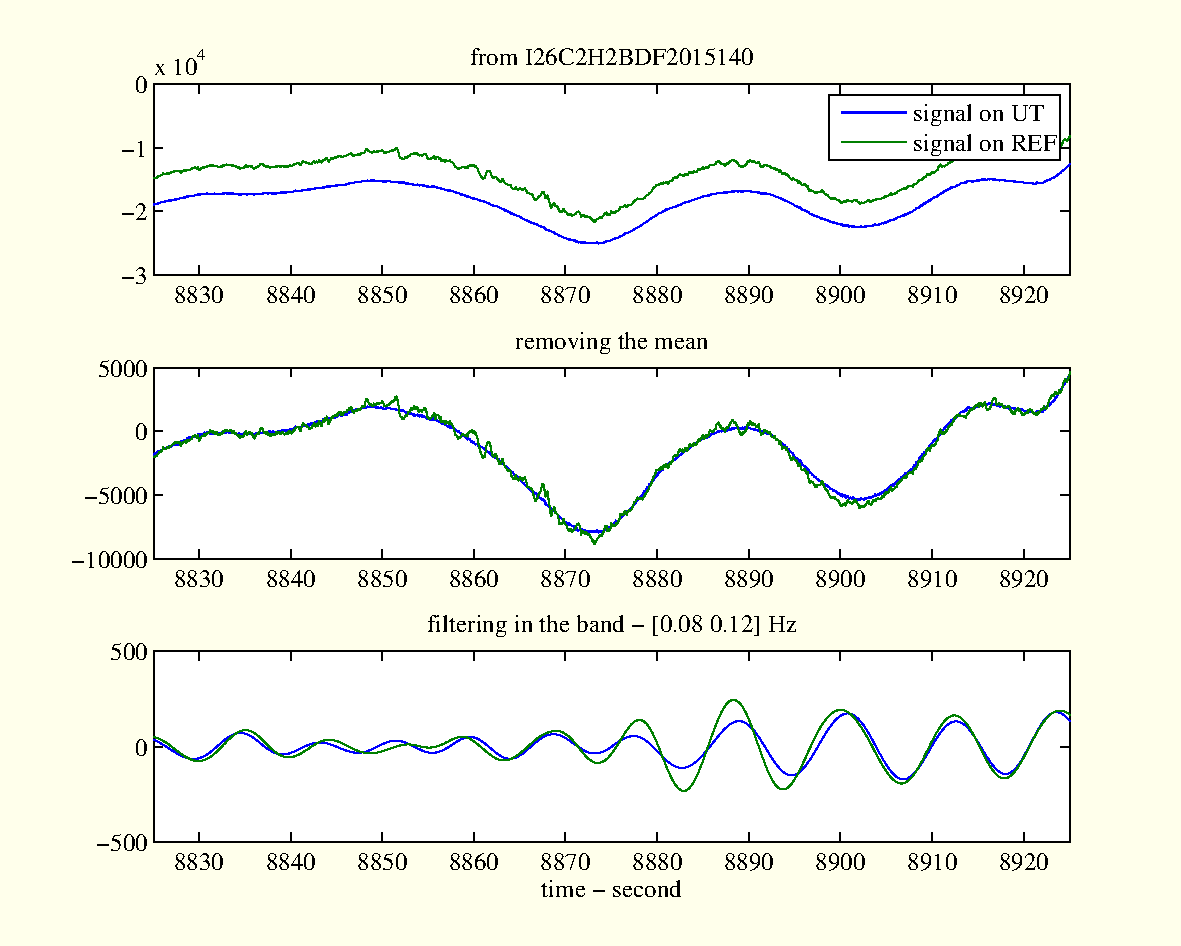
\includegraphics[scale=0.5]{signalsanomaly.pdf}
\end{minipage}
\begin{minipage}[c]{8cm}
              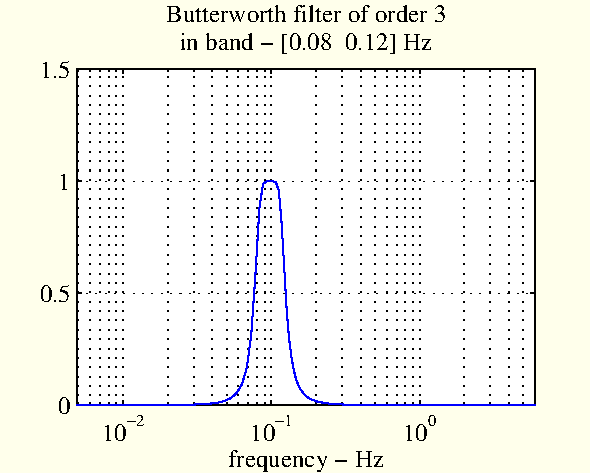
\includegraphics[scale=0.5]{filteranomaly.pdf}    

\end{minipage}
\centering
\caption{Filtered signals}
\label{fig:filteredsignals}
\end{figure}

